\section{Sets of equations}
    General systems of $N$ non-linear functions $f_i(\Vec{x})$, $i=1,\dots,N$, where $\Vec{x}= (x_1, \dots, x_M)^\top$ is a vector of $M$ unknowns. Find $\Vec{x}^\star$, st. $f_i(\Vec{x}^\star) = 0 \quad i = 1,\dots,M$
    
    We define the \textit{Jacobian Matrix} $J(\Vec{x})$ with elements $J_{ij}(\Vec{x}) = \frac{\partial f_i(\Vec{x})}{\partial x_j}$
    \begin{equation*}
        J(\Vec{x}) = 
        \begin{bmatrix}
            \frac{\partial f_1(\Vec{x})}{\partial x_1} & \frac{\partial f_1(\Vec{x})}{\partial x_2} & \dots & \frac{\partial f_1(\Vec{x})}{\partial x_M}\\
            \frac{\partial f_2(\Vec{x})}{\partial x_1} & \frac{\partial f_2(\Vec{x})}{\partial x_2} & \dots & \frac{\partial f_2(\Vec{x})}{\partial x_M}\\
            \vdots & \vdots & \ddots & \vdots\\
            \frac{\partial f_N(\Vec{x})}{\partial x_1} & \frac{\partial f_N(\Vec{x})}{\partial x_2} & \dots &  \frac{\partial f_N(\Vec{x})}{\partial x_M}
        \end{bmatrix}
    \end{equation*}
    
    \subsection{Condition Number}
        For a system of $N$ non-linear equations and $M$ unknowns the condition number of the root finding problem for the root $\Vec{x}^\star$ of $F$ is $\|J^{-1}(\Vec{x}^\star)\|$
    
    \subsubsection{Newtons Method}
    If we set $\Vec{x}_{k+1} = \Vec{x}_k + \Vec{z}$ we have to solve $A\Vec{z} = \Vec{b}$ at every step with $A = J(\Vec{x}_k)$ and $\Vec{b} = -F(\Vec{x}_k)$
    \begin{gather*}
        \mathbf{0}=F(\Vec{x}^\star) \approx F(\Vec{x}_k) + J(\Vec{x}_k)(\Vec{x}^\star -\Vec{x}_k)\\
        J(\Vec{x}_k)(\Vec{x}_{k+1} - \Vec{x}_k) = -F(\Vec{x}_k)
    \end{gather*}
    
    \textbf{Netwon-Raphson Method (\textit{N} = \textit{M}):}
    \begin{equation*}
        \colorboxed{red}{\Vec{x}_{k+1} = \Vec{x}_k - J^{-1}(\Vec{x}_k)F(\Vec{x}_k)} \ 
        \colorboxed{red}{
    \begin{aligned}
    J(\Vec{x}_k)\Vec{z} &= -F(\Vec{x}_k)\\
    \Vec{x}_{k+1} &= \Vec{x}_k + \Vec{z}
    \end{aligned}
    }
    \end{equation*}
    % We do not invert $J(\Vec{x}_k)$ but solve \begin{equation*}
    % \colorboxed{red}{
    % \begin{aligned}
    % J(\Vec{x}_k)\Vec{z} &= -F(\Vec{x}_k)\\
    % \Vec{x}_{k+1} &= \Vec{x}_k + \Vec{z}
    % \end{aligned}
    % }
    % \end{equation*}
    % J(\Vec{x}_k)\Vec{z} = -F(\Vec{x}_k)\Vec{x}_{k+1} = \Vec{x}_k + \Vec{z}
    
    Provided that the Jacobian is not singular the convergence rate is quadratic.
    
    \textbf{Pseudo-Newton Method (\textit{N}$\neq$\textit{M}):}
    \begin{equation*}
        \colorboxed{red}{\Vec{x}_{k+1} = \Vec{x}_k - J^{+}(\Vec{x}_k)F(\Vec{x}_k)}
    \end{equation*}
    Assuming J always has full rank
    
    \begin{center}
        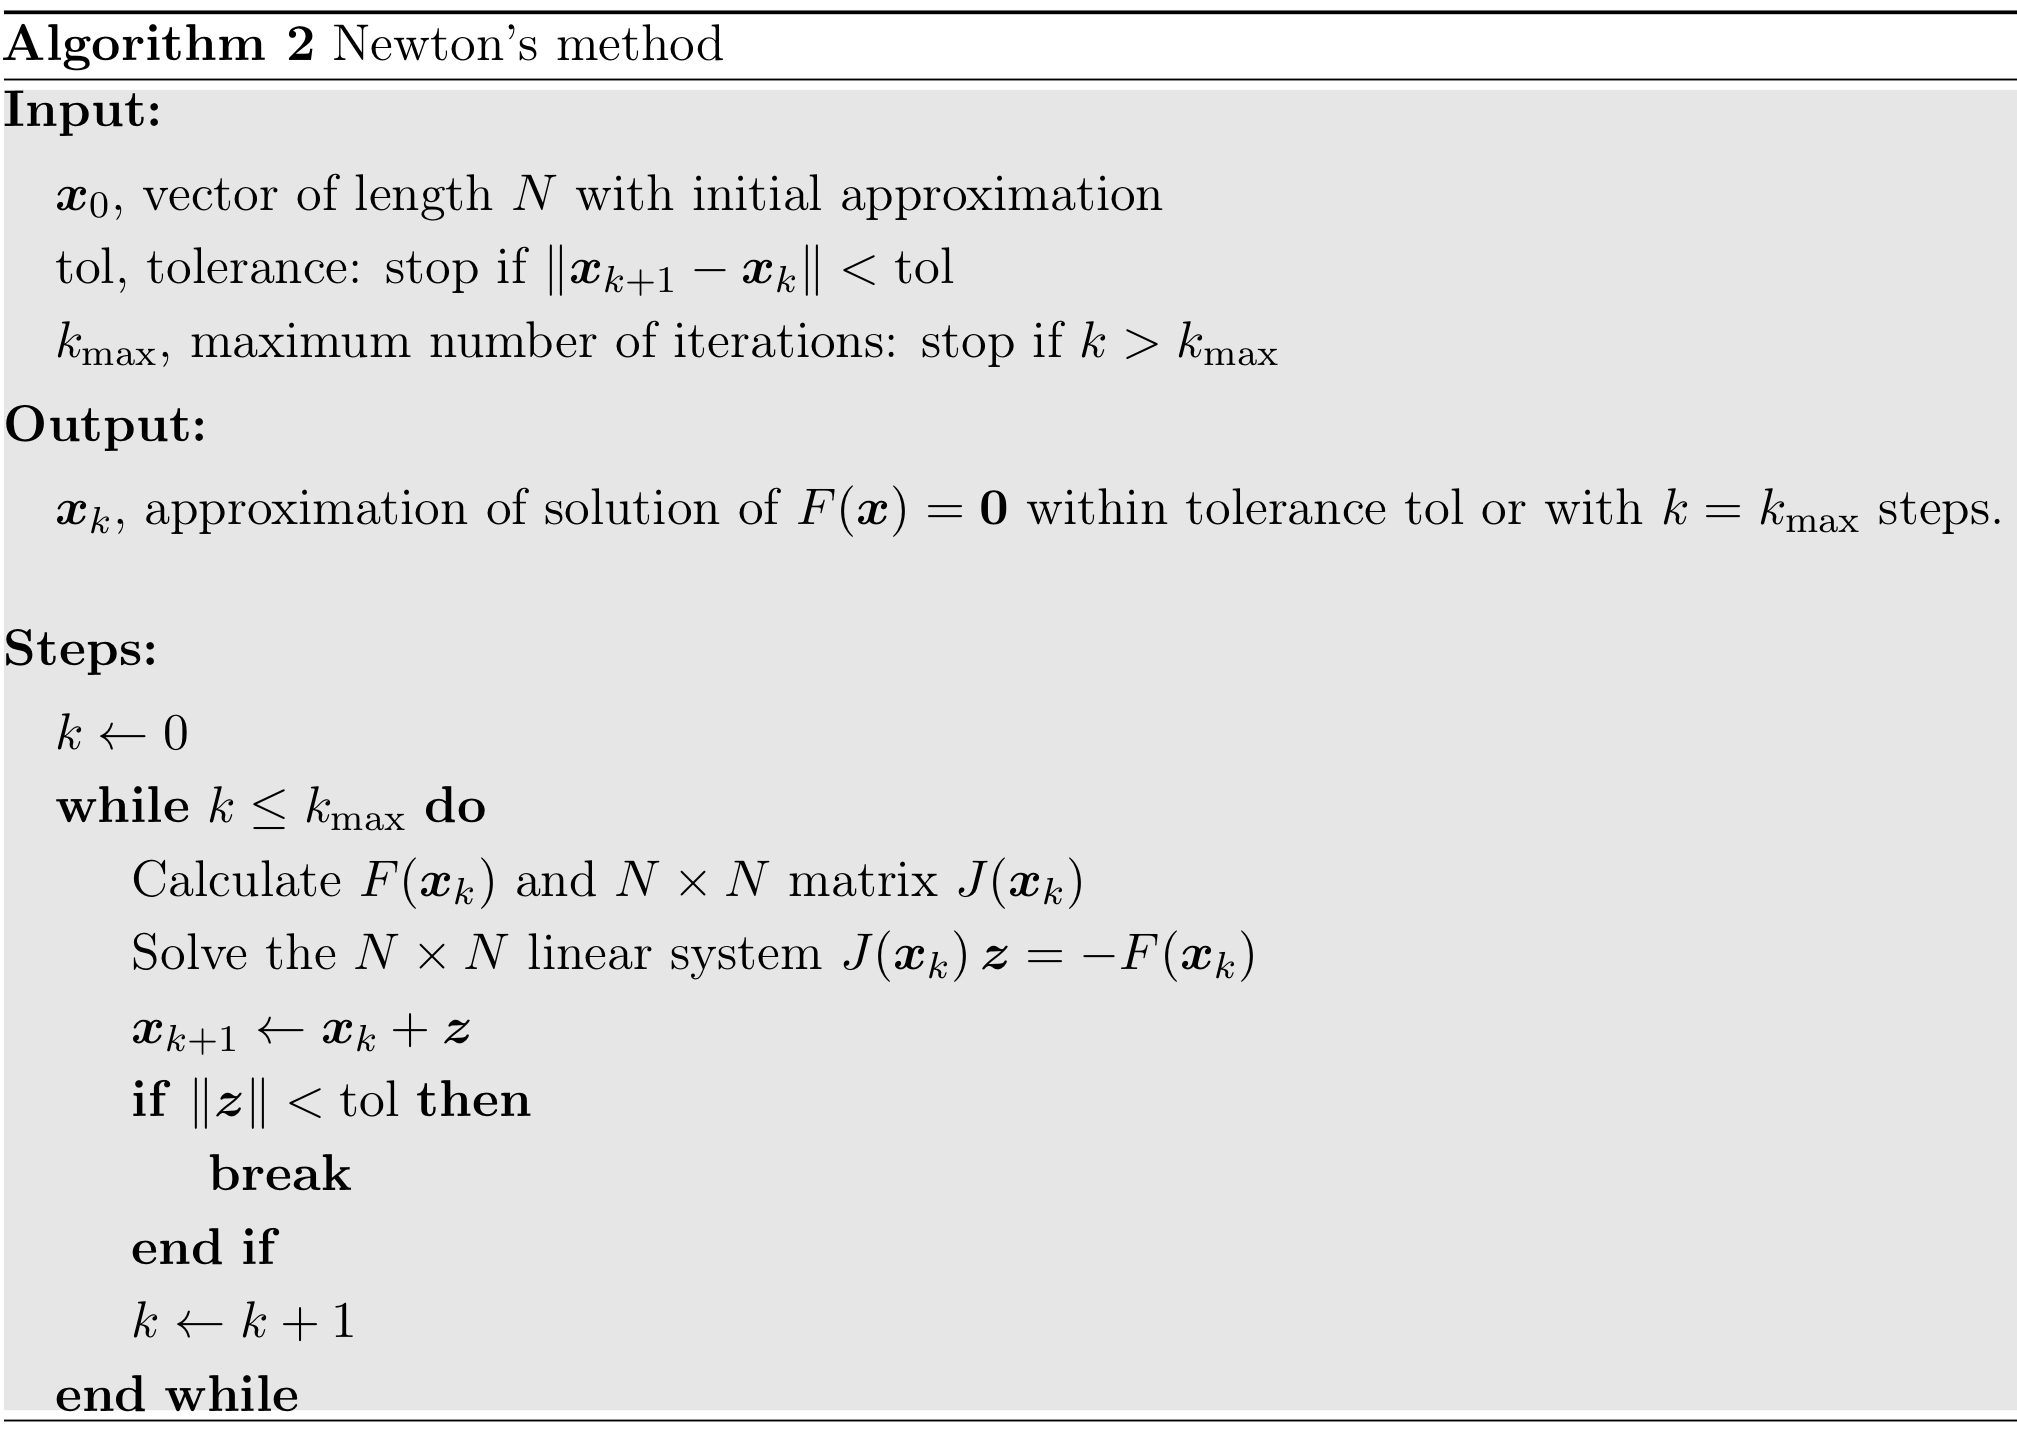
\includegraphics[width = \linewidth]{images/02/soe_newtons_meth.jpeg}
    \end{center}